\documentclass[10pt,twocolumn,letterpaper]{article}

\usepackage{cvpr}
\usepackage{times}
\usepackage{epsfig}
\usepackage{graphicx}
\usepackage{amsmath}
\usepackage{amssymb}
\usepackage{booktabs}
\usepackage{subcaption}

\def\tightlist{}

% Include other packages here, before hyperref.

% If you comment hyperref and then uncomment it, you should delete
% egpaper.aux before re-running latex.  (Or just hit 'q' on the first latex
% run, let it finish, and you should be clear).
\usepackage[pagebackref=true,breaklinks=true,letterpaper=true,colorlinks,bookmarks=false]{hyperref}

\cvprfinalcopy % *** Uncomment this line for the final submission

\def\cvprPaperID{****} % *** Enter the CVPR Paper ID here
\def\httilde{\mbox{\tt\raisebox{-.5ex}{\symbol{126}}}}

% Pages are numbered in submission mode, and unnumbered in camera-ready
\ifcvprfinal\pagestyle{empty}\fi
\begin{document}

%%%%%%%%% TITLE
\title{Machine-Oriented Compression}

\author{Natalia Frumkin\\
The University of Texas at Austin\\
{\tt\small nfrumkin@utexas.edu}
% For a paper whose authors are all at the same institution,
% omit the following lines up until the closing ``}''.
% Additional authors and addresses can be added with ``\and'',
% just like the second author.
% To save space, use either the email address or home page, not both
\and
Dan Jacobellis\\
The University of Texas at Austin\\
{\tt\small danjacobellis@utexas.edu}
}

\maketitle

%%%%%%%%% BODY TEXT

\begin{abstract}
Despite significant advances in neural network-based lossy compression, most machine learning datasets and inference pipelines still utilize the decades old JPEG and MPEG standards with compression ratios of only about 5:1.  In this work, we compare two approaches for utilizing neural compression in machine perception systems: (1)~full-input compression, and (2)~model-splitting. In the full-input approach, the reconstruction objective is fully decoupled from downstream tasks, and we find that minimal loss in downstream performance on common tasks--- including classification and segmentation---can be achieved even with compression rates exceeding 500:1. However, since these more potent neural compression systems discard and re-synthesize details, such as texture, faces and text, there is a concern that downstream performance on fine-grained perception tasks could suffer. In the second approach, model-splitting, this loss is avoided by applying the task encoder directly to the the original image, which additionally benefits from simplified inference. We show that the representations derived from two recent self-supervised pre-training methods, DINO and BEiT, can be combined with the model splitting approach to achieve better performance at a lower data rate than the conventional approach of full-input JPEG processing. We make our code and experiments publicly available
\footnote{\href{https://github.com/danjacobellis/MPQ}{github.com/danjacobellis/MPQ}}
\footnote{\href{https://github.com/nfumkin/BEiT-compress}{github.com/nfumkin/BEiT-compress}}
\footnote{\href{https://github.com/danjacobellis/CMMR}{github.com/danjacobellis/CMMR}}.

\end{abstract}

\begin{figure}[t]
\begin{center}
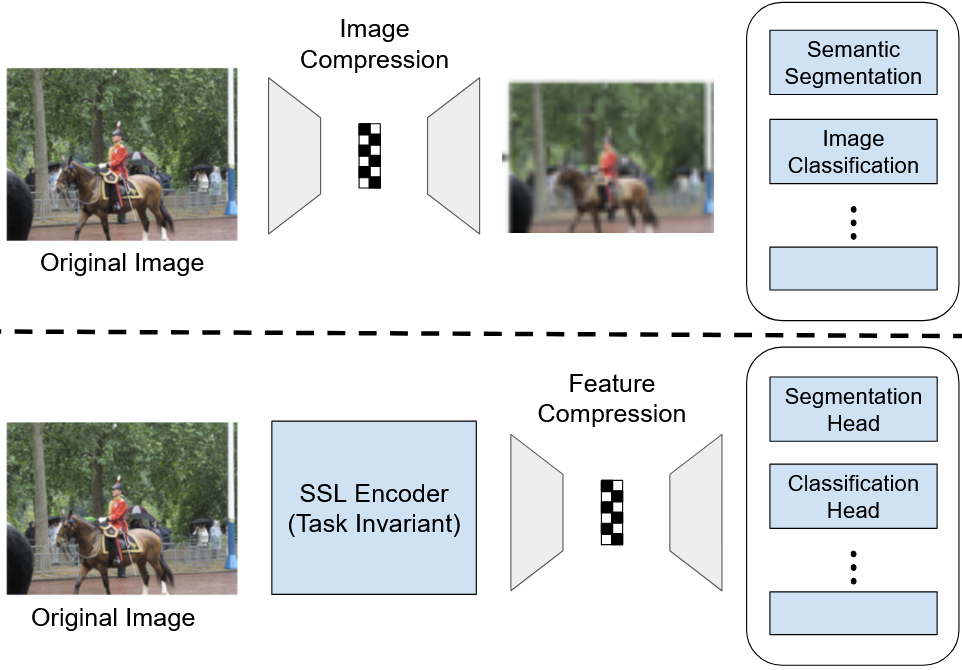
\includegraphics[width=0.5\textwidth]{Figures/compression-pipelines.png}
\end{center}
\caption{\label{fig:compression-pipelines}%
Compressed domain learning pipelines usually apply image compression \textit{as a pre-processing step} for downstream vision tasks (pipeline on top). In this project, we consider feature compression for existing SSL representations and use a compressed feature representation for a variety of SSL decoders (bottom pipeline).}
\end{figure}

\begin{figure*}
\begin{center}
\epsfig{width=6.0in,file=Figures/image_compression_methods}
\end{center}
\caption{\label{fig:image_compression_methods}%
Visual comparison of image compression methods. Best viewed zoomed in.}
\end{figure*}


\section{Introduction}

In contemporary machine perception pipelines, lossy compression techniques are often employed, but using legacy codecs at near-lossless quality levels, thus limiting potential savings in data rate~\cite{ehrlich2022first}. For instance, the ImageNet dataset, a cornerstone for image classification tasks, utilizes JPEG compression with an average compression ratio of roughly 5:1. As a result, the full ImageNet-21k is over 1.3 TB in size, and common practice is to discard most of this information using a 224x224 reduced resolution version~\cite{ridnik2021imagenet}. Additionally, many types of sensors necessitate extremely high compression ratios, sometimes exceeding 1000:1~\cite{cocker2022low}, resulting from high resolution measurements combined with limited communication bandwidth. As a result, vast amounts of rich, high-fidelity data captured by modern sensors are underutilized or even discarded entirely.

In the decades since the introduction of the ubiquitous JPEG and MPEG standards for images and audio, advancements in lossy compression technologies have demonstrated the capability to achieve high compression ratios with minimal degradation in quality. For example, it has been shown that storing the ImageNet-1k dataset using the tokens produced by a ViT-VQGAN neural compression model saves a factor of 100:1 in storage and leads to faster and simplified training ~\cite{yu2021vector}\cite{park2023storage}. 
While the advantages of employing more potent lossy compression techniques are evident, uncertainty surrounding their impact on downstream machine perception tasks remains a significant barrier. For example, Ilyas et al.,~\cite{ilyas2019adversarial} demonstrate the existence of signal components, called non-robust features, which are highly predictive yet imperceptible to humans. Lossy compression during training is likely to eliminate these features and thereby lead to sub-optimal models~\cite{aydemir2018effects}. Additionally, failure to match the exact lossy compression method and settings during training and inference could lead to distribution shift and unpredictable model behavior.

While the evaluation of human perceptual quality has been extensively studied, it is less clear how different types lossy compression affect the performance of downstream models. Ongoing codec development efforts aim to optimize for machine perception, a paradigm referred to as ``compression for machines~\cite{chamain2021end}" or ``machine-oriented compression~\cite{kang2023super}."  Most notably, The JPEG AI standard \cite{ascenso2023jpeg} proposes a single stream image encoder supporting multiple decoders for both human and machine perception. Harell et al.,~\cite{harell2023rate} proposed a taxonomy of three different machine-oriented compression approaches. Notable to our work is the method of full-input machine-oriented compression, where the signal is fully decoded before performing downstream tasks, and the model-splitting approach, where intermediate features are compressed rather than the original signal. Our contributions are twofold:

\begin{itemize}
\item \textit{Evaluation of Existing Full-Input Methods}: We systematically evaluate the impact of various types of lossy compression---both conventional and neural---on audio and visual machine learning tasks using the full-input approach. Our results in this area indicate three key findings: (1) using generative compression, it is feasible to leverage highly compressed data while incurring a negligible impact on machine perceptual quality; (2) machine perceptual quality correlates strongly with deep similarity metrics, indicating a crucial role of these metrics in the development of machine-oriented codecs; and (3) using lossy compressed datasets, (e.g. ImageNet) for pre-training can lead to counter-intuitive scenarios where lossy compression increases machine perceptual quality rather than degrading it.
\item \textit{Feature Compression on SSL Representations}: We combine the model-splitting approach, which typically focuses on a single task, with self-supervised pre-training, which produces general-purpose representations. While the standard approach to model splitting increases the efficiency of inference, exploiting the complementary properties of neural compression and self-supervised learning (SSL) also allows us to also vastly simplify training of downstream tasks. We consider model-splitting for DINOv2 and BeiT-2 and are able to achieve compression ratios of 588:1 and 7:1 for image classification and segmentation respectively.
\end{itemize}
\begin{table}[ht]
\centering
\caption{Summary of Datasets and Models used for Full-Input Compression}
\label{tab:datasets_models}
\begin{tabular}{llll}
\toprule
Dataset & Task Type & Model & Metric \\
\midrule
ImageNet-1k & Classification & ViT &  Acc. \\
ChestX-ray8 & Classification & ViT & Acc. \\
Bean Disease & Classification & ViT & Acc. \\
ADE20k & Segmentation & SegFormer & mIOU \\
Common Voice & Recognition & Whisper & WRA \\
MUSDB-HQ & Separation & Demucs v3 & SDR \\
\bottomrule
\end{tabular}
\end{table}

\begin{table}[ht]
\centering
\caption{Summary of Compression Methods}
\label{tab:compression_methods}
\begin{tabular}{lll}
\toprule
Method & Description & Setting \\
\midrule
JPEG & DCT-based coding & Quality: 5 \\
WEBP & Transform coding & Quality: 0 \\
MBT2018 & Neural compression & Quality: 1 \\
HiFiC & Generative compression & Quality: Low \\
MP3 & Audio coding & Bitrate: 8 kbps \\
Opus & Audio compression & Bitrate: 6 kbps \\
EnCodec & Neural audio compression & Bitrate: 6 kbps \\
\bottomrule
\end{tabular}
\end{table}


\section{Machine Perceptual Quality Under Full-Input Compression}

We investigate the impact of different audio and image compression techniques on machine perceptual quality under severe lossy compression---which we define as ratios compression ratios between 20:1 and 1000:1---and compare against a baseline that does not have additional compression. We employ six datasets, seven different lossy compression methods, and use popular pre-trained models for various discriminative tasks as summarized in Tables \ref{tab:datasets_models} and \ref{tab:compression_methods}. We use the performance on the validation split of each dataset as a measure of machine perceptual quality. We evaluate the compression performance based on bitrate, conventional distortion metrics, and deep similarity metrics. 

\paragraph{Models and datasets.} We employ the ImageNet-1k dataset for image classification, using a vision transformer (ViT) pre-trained on ImageNet-21k ~\cite{dosovitskiy2020image}. The NIH ChestX-ray8 dataset ~\cite{wang2017chestx} for pneumonia classification and the bean disease dataset \cite{singh2023classification} are also used in conjunction with an ImageNet-21k pre-trained ViT. Semantic segmentation is performed on the ADE20k dataset \cite{zhou2017scene} using the SegFormer model \cite{xie2021segformer}. The Common Voice 11.0 dataset \cite{ardila2020common} and the Whisper model \cite{radford2023robust} are used for speech recognition. Finally, the MUSDB-HQ dataset, an uncompressed version of MUSDB18 \cite{rafii2017musdb18}, and the Demucs v3 model \cite{defossez2021hybrid} are used for music source separation. These datasets and corresponding models are summarized in Table \ref{tab:datasets_models}.

\paragraph{{Compression methods}}The image compression methods in our study include JPEG, WEBP, the distortion-optimized neural compression approach from Minnen et al. ~\cite{minnen2018joint} , and the generative compression method HiFiC ~\cite{mentzer2020high}. For audio compression, we use MPEG Layer III (MP3), Opus, and the neural audio model EnCodec \cite{defossez2022high}. Table \ref{tab:compression_methods} summarizes these methods. Additional implementation details and a listing of specific model variants are available in our code repository~\footnote{\href{https://github.com/danjacobellis/MPQ}{Github: danjacobellis/MPQ}}.

\paragraph{Evaluation metrics.} We use conventional rate-distortion metrics as well as deep similarity metrics---quality metrics derived from deep neural networks and trained to predict human judgments of quality. Each metric is calculated on a per-sample basis.
\begin{itemize}

\item \textit{Bits Per Pixel (BPP)} and \textit{Bits Per Sample (BPS)} are used to measure the rate of images and audio signals respectively. For the EnCodec model, which supports a default mode where the VQVAE codes are directly stored and a secondary mode that uses additional entropy coding, we use the default mode without entropy coding and calculate BPS using the the product of the codebook size and the number codes. For all other codecs, we directly measure the rate based on the size of the encoded file.

\item \textit{Peak Signal-to-Noise Ratio (PSNR)} is used as a conventional distortion metric for both images and audio. We represent image signals using the range $[0,255]$ and represent audio signals using the range $[-1,1]$, so \( \text{PSNR} = 20\log_{10}(255) - 10\log_{10}(\text{MSE}) \) for images and \( \text{PSNR} = -10\log_{10}(\text{MSE}) \) for audio.

\item \textit{Learned Perceptual Image Patch Similarity (LPIPS)}\cite{zhang2018unreasonable} is a deep similarity metric specifically designed for images. It captures complex perceptual differences that simpler metrics like PSNR or SSIM are insensitive to. In the table, we report \( -10\log_{10}(\text{LPIPS similarity}) \) to align it with the other quality metrics.

\item  \textit{Contrastive Deep Perceptual Audio Similarity Metric (CDPAM)} \cite{manocha2021cdpam} is a deep similarity metric is designed for audio. Like LPIPS for images, it captures perceptual differences more effectively than PSNR. Similar to LPIPS, we report \( -10\log_{10}(\text{CDPAM similarity}) \).
\end{itemize}


\begin{figure}
\begin{center}
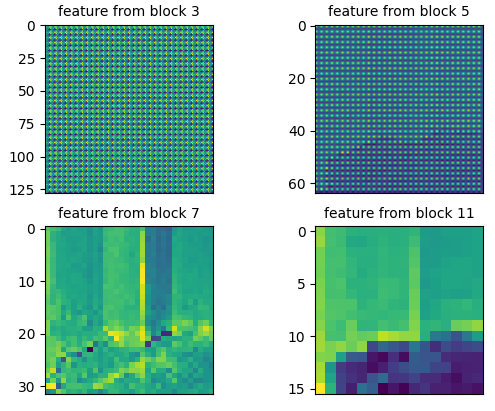
\includegraphics[width=0.5\textwidth]{Figures/img0_patch0.png}
\end{center}
\caption{\label{fig:beit-features}%
A sample of BeiT-2 features. The uncompressed feature representation consists of four features (the output feature maps of attention blocks 3,5,7, and 11). For compression, we consider applying vector quantizers on this representation directly, as well as element-wise addition of all four feature maps to compress by 4X.}
\end{figure}

\section{Model-Splitting Based Compression}

Existing self-supervised pre-training methods including MoCo~\cite{chen2021empirical}, BYOL~\cite{grill2020bootstrap}, BeiT~\cite{peng2022beit}, and DINO~\cite{oquab2023dinov2} produce strong feature representations for a variety of downstream tasks. Once pre-trained, the learned encoders can be used for a variety of task-specific decoders. We leverage these powerful SSL encoders for model-splitting compression by applying feature compression on existing SSL encoder features, allowing us to reuse the same compressed representation for all task-specific decoders. To compress these representations, we consider a variety of quantization technieques and rate-distortion autoencoders as outlined below. 

\textbf{Scalar Quantization} Standard post-training quantization is often applied to model features for fast inference and reduced model size~\cite{wu2020integer}. These post-training techniques can be similarly applied to the SSL features to achieve high compression ratios. In this work, we will consider uniform quantization for a variety of different bit-widths, INT8, INT4, and INT2, represented in the following form:

\begin{equation}
  Q(\textbf{x}, \delta, b) = \texttt{clip}(\Big{\lfloor} \frac{\textbf{x}}{\delta} \Big{\rceil}, -2^{b-1}+1, 2^{b-1}-1)
  \label{eq:quant}
\end{equation}

where $\delta$ is the scale parameter analytically computed using MinMax quantization~\cite{jacob2018quantization}, $b$ is bit-width (8,4, or 2) and $\textbf{x}$ is the original 32-bit floating point value.

\textbf{Learned Vector Quantization} Learned vector quantizers (VQ)~\cite{van2017neural} can achieve better performance to scalar quantization, and are widely used for both audio~\cite{defossez2022high} and image ~\cite{Duan_2023, el-nouby2023image} compression. Recently, Finite Scalar Quantization (FSQ)  has shown improved performance over standard VQ-VAE representations~\cite{mentzer2023finite}. In particular, FSQ is more robust to codebook collapse since it's implicit codebook representation allows better codebook utilization and removes the auxiliary losses present for standard VQ-VAE style vector codebooks.

\textbf{Rate-Distortion Autoencoder (RDAE)} While learned vector quantization compresses signals by using a low-dimensional codebook, an alternative approach is construct a differentiable approximation entropy of an intermediate layer, so that the rate-distortion function $R+\lambda D$ can be directly optimized~\cite{balle2017end}. The distortion function can be any differentiable or similarity metrics, such as MSE, SSIM, or LPIPS.  Once the latent feature has minimal entropy, it can be compressed using a lossless data compression method such as Huffman coding or arithmetic coding. For compressing, DINO features, we constructed RDAEs with symmetric analysis and sythesis transforms and optimized them for MSE reconstruction using $\lambda=0.1$. We tested two archetectures; a high-rate variant with two analysis layers and $2\times$ spatial downsampling in each dimension, and a high-rate variant with three analysis and and $4\times$ spatial downsampling.

We consider scalar quantization, vector quantizers, and rate-distortion autoencoders for SSL feature compression. Scalar quantization is applied in a post-training manner, whereas the vector quantizer and RDAEs are fine-tuning in conjunction with the downstream decoders. Sections \ref{sec:model-splitting-results} will evaluate these compression methods on two popular SSL representations.
% \textbf{Feature Compression Approach}.
% Due to the inherent limits of full-input machine-oriented compression, we investigate an alternative architecture based on feature compression. We compute the embeddings produced by BeiT-2, a self-supervised vision transformer that is known to generate representations that transfer effectively to a variety of tasks, including image classification and segmentation \cite{peng2022beit}. While these representation are known to be effective for downstream tasks, they are considerably larger than the corresponding compressed image. To mitigate this, we explore the training of a neural compression model specifically tailored to these high-dimensional features \cite{singh2020end}. Our codec is based on Finite Scalar Quantization (FSQ), a simplified variant of the VQ-VAE. \cite{mentzer2023finite}.



\begin{figure*}
\begin{center}
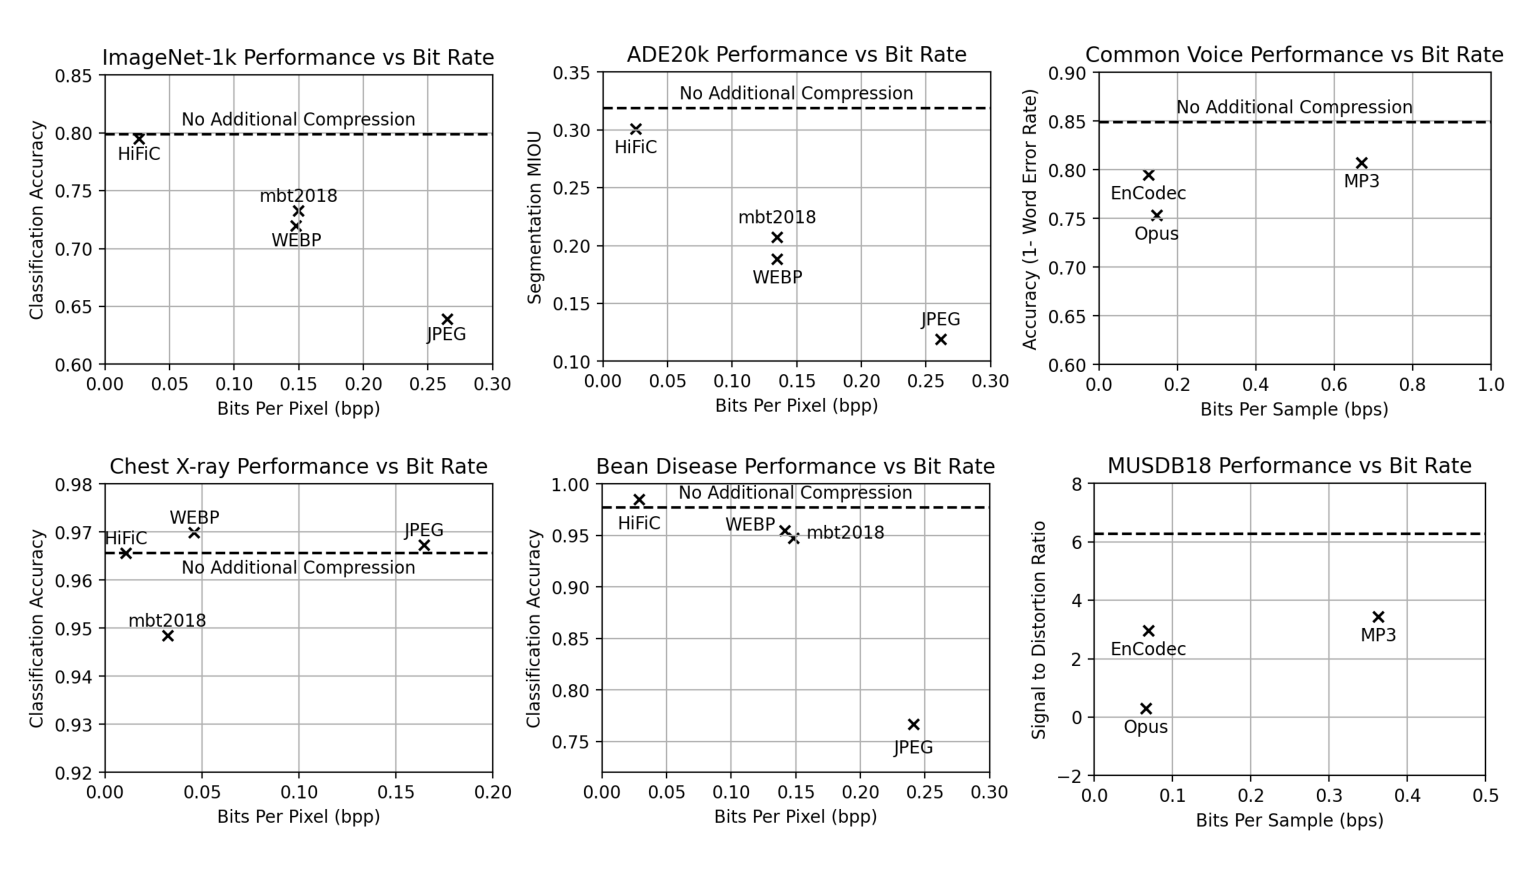
\epsfig{width=6.0in,file=Figures/mpq_results}
\end{center}
\caption{\label{fig:mpq_results}%
Performance on various machine perception tasks under full-input machine coding.}
\end{figure*}

\begin{table*}[!htb]
    \caption{Comparing Compression \& Machine Perceptual Quality across Various Techniques}
    \label{tab:compression_comparison}
        \begin{subtable}{.6\linewidth}
      \centering
        \caption{Summary of Image Results}
        \label{tab:image_compression_comparison}
        \setlength{\tabcolsep}{3pt}
        {\small\begin{tabular}{lcccccc}
\toprule
Metric & Dataset & Baseline & JPEG & WEBP & MBT & HiFiC \\
\midrule
PSNR & ImageNet &  & 23.2 & 24.8 & \textbf{26.7} & 26.3 \\
     & ADE20k &  & 23.9 & 25.6 & \textbf{28.1} & 27.7 \\
     & Bean &  & 20.8 & 22.0 & \textbf{22.9} & 21.8 \\
     & X-ray &  & 30.0 & 32.7 & 34.7 & \textbf{36.4} \\
\midrule
LPIPS & ImageNet &  & 6.11 & 7.02 & 7.95 & \textbf{10.8} \\
      & ADE20k &  & 7.13 & 7.96 & 8.99 & \textbf{11.8 }\\
      & Bean &  & 5.72 & 6.75 & 6.90 & \textbf{9.78} \\
      & X-ray &  & 6.85 & 7.58 & 7.80 & \textbf{13.2} \\
\midrule
BPP & ImageNet &  & \textbf{0.26} & 0.148 & 0.150 & 0.026 \\
    & ADE20k &  & \textbf{0.26} & 0.14 & 0.14 & 0.025 \\
    & Bean &  & 0.24 & 0.14 & 0.15 & \textbf{0.029} \\
    & X-ray &  & \textbf{0.17} & 0.046 & 0.032 & 0.011 \\
\midrule
Top-1 & ImageNet & \textbf{0.799} & 0.639 & 0.720 & 0.733 & 0.795 \\
 Accuracy                        & Bean & 0.977 & 0.767 & 0.955 & 0.947 &\textbf{ 0.985} \\
                        & X-ray & 0.966 & 0.967 & \textbf{0.970} & 0.948 & 0.966 \\
\midrule
mIOU & ADE20k & \textbf{0.319} & 0.119 & 0.189 & 0.208 & 0.301 \\
\bottomrule
\end{tabular}}
    \end{subtable} 
    \begin{subtable}{.4\linewidth}
      \centering
        \caption{Summary of Audio Results}
        \label{tab:audio_compression_comparison}
         \setlength{\tabcolsep}{3pt}
        {\small\begin{tabular}{lccccc}
        \toprule
        Metric & Dataset & Baseline & MP3 & OPUS & EnCodec \\
        \midrule
        PSNR & MUSDB18 &  &\textbf{ 29.17} & 22.17 & 24.95 \\
             & CV &  & \textbf{33.89} & 26.70 & 29.04 \\
        \midrule
        CDPAM & MUSDB18 &  & 38.43 & 36.46 & \textbf{45.33} \\
              & CV &  & 37.89 & 38.27 & \textbf{46.34} \\
        \midrule
        BPS & MUSDB18 &  & \textbf{0.36} & 0.066 & 0.069 \\
            & CV &  & \textbf{0.67} & 0.14 & 0.13 \\
        \midrule
        SDR & MUSDB18 & \textbf{6.29} & 3.44 & 0.30 & 2.97 \\
        \midrule
        WRA & CV & \textbf{0.85} & 0.81 & 0.75 & 0.80 \\
        \bottomrule
        \end{tabular}}
    \end{subtable}%
\end{table*}

\section{Results of Full-Input Compression}
\label{sec:full-input-results}
Our evaluation across multiple datasets and machine perception tasks reveals key insights into the impact of lossy compression on machine perceptual quality. The results are shown in Figure~\ref{fig:mpq_results} and are summarized in Tables~\ref{tab:image_compression_comparison} and~\ref{tab:audio_compression_comparison}. For image-based tasks, LPIPS is a better predictor of downstream performance than PSNR, and generative compression (HiFiC) performs the best at all but one of the tasks (Chest X-ray) despite having the lowest average bitrate, and consistently achieves results close to the uncompressed baseline. In the audio domain, similar trends are observed; the audio quality measured by CDPAM is better predictor of downstream performance than PSNR, and, among the methods tested, EnCodec provides the best trade-off between rate and downstream performance for both datasets.

\begin{table*}
\centering
\caption{Feature Compression Results using BeiT-2}
\label{tab:feature_compression_results}
\begin{tabular}{l|ccccc}
\toprule
Downstream Task & Compression Scheme & Finetune All & Finetune Task Layer Only & BPP & Compression Ratio \\
\midrule
% \multicolumn{5}{c}{BeiT Image Classification} \\
\cmidrule(lr){1-5}
BeiT Image & None & 86.4 & 86.2 & 0.490 & 49 \\
  Classification & with 8-bit FSQ & \textbf{87.7} & \textbf{87.7} & 0.041 & 588 \\
(\textbf{Top-1 Accuracy}) &INT8 Quantized Code & 86.4 & 86.1 & 0.122 & 196 \\
&INT2 Quantized Code & 85.4 & 85.2 & \textbf{0.031} & \textbf{784} \\
\midrule
% \multicolumn{5}{c}{BeiT Semantic Segmentation} \\
\cmidrule(lr){1-5}
BeiT Semantic & None & 53.5 & 53.0 & 384 & 0.0625 \\
 % & with 32-bit FSQ & - & 52.18 & 128 & 0.1875 \\
 Segmentation & 8-bit FSQ & - & 41.65 & 32 & 0.75 \\
(\textbf{mIOU})  & element-wise add & - & \textbf{54.74} & 96 & 0.25 \\
  &  element-wise add + FSQ & - & 53.15 & \textbf{8} & \textbf{3} \\
\bottomrule
\end{tabular}
\end{table*}

\section{Results of Model-Splitting Compression}
\label{sec:model-splitting-results}
\textbf{Experimental Setup} We consider two SSL encoders for model-splitting compression: DINOv2~\cite{oquab2023dinov2} and BeiT-2~\cite{peng2022beit}. Both models use a pre-trained SSL encoder (ex: ViT-Base) and subsequently learn specialized decoders for downstream tasks. All downstream tasks share a feature representation (the output of the SSL encoder) which we will apply feature compression on. We consider two representative downstream tasks: image classification, which requires knowledge of scene representations, and semantic segmentation, which requires semantic understanding and boundary detection. We report ImageNet-1k Top-1 accuracy and mIOU for classification and segmentation respectively. BeiT-2 fine-tuning requires significant computational resources; Image classification fine-tuning requires 0.75 days and semantic segmentation takes 1.5 days on eight Nvidia A5000 GPUs. 

\textbf{BeiT-2 Compression}
% Naturally, semantic segmentation's feature space must be more 
As shown in Table~\ref{tab:feature_compression_results}, utilizing FSQ allows us to achieve a high compression rate with no loss in classification accuracy. Surprisingly, post-training quantization does not degrade performance sharply, and offers extremely high compression ratios. Quantizing to INT2 yields a compression ratio of 784X with only a 1.2\% drop in accuracy. For semantic segmentation, we are presented with a significant compression challenge -- the encoder generates a large intermediary representation (size is [4,768,32,32]) which leads to a 384 bits-per-pixel. For image classification, we are able to directly use the pooled feature representation from attention block 11, whereas the BeiT-2's segmentation decoder requires the four pre-pooled feature representations shown in Figure~\ref{fig:beit-features}. Applying 8-bit FSQ as done with image classification generates a whopping 32 bits per pixel (expansion, not compression). To achieve compression, we combine the four pre-pooled representations using a element-wise add and find that this representation yields better performance than baseline (+1.24 mIOU). Combining element-wise add and 8-bit FSQ, we achieve a compression ratio of 3X with -0.35 mIOU degradation.

\begin{table}
\centering
\caption{DINO Compression Results}
\label{tab:dino_compression_results}
\begin{tabular}{l|cccc}
\toprule
Task & RDAE & Linear & BPP & Ratio \\
\midrule
% \multicolumn{5}{c}{DINO Image Classification} \\
\cmidrule(lr){1-5}
INet-1k Acc. & None & 86.4 & 250.8 & 1:10 \\
& 4x & 85.5 & 16.0 & 7:1 \\
\midrule
% \multicolumn{5}{c}{DINO Semantic Segmentation} \\
\cmidrule(lr){1-5}
ADE20k mIOU & None & 42.2 & 250.8 & 1:10 \\
& 2x & 39.2 & 16.0 & 1.5:1 \\
& 4x & 32.1 & 3.5 & 7:1 \\
\bottomrule
\end{tabular}
\end{table}


\textbf{DINOv2 Compression} We train RDAEs to compress the patch tokens produced by DINOv2. The results are shown in Table~\ref{tab:dino_compression_results}. We use the Vimeo90k dataset~\cite{xue2019video} at $448\times252$ resolution and train RDAEs on the corresponding patch tokens (size $1536\times32\times18$). For both the $2\times$ and the $4\times$ variant, we use symmetric analysis and synthesis transforms with 4096 channels in each intermediate layer, which consists of 5x5 convolution, 2x downsampling and generalized divisive normalization (GDN)~\cite{johnston2019computationally}, while the input and 
output layers are $1x1$ convolutions without downsampling. To reduce the parameter count, we split the channels into 32 groups, resulting in 32 filters of size $128\times5\times5$ in each layer. We use the same linear probing technique to perform classification and segmentation as in the original DINOv2 paper~\cite{oquab2023dinov2}. The linear heads are only trained once on the uncompressed inputs, and are never fine-tuned on the compressed variants.  While the downstream performance is reduced compared to the BEiT/FSQ model, Our DINO/RDAE combination requires significantly less training resources, both for the compression model and the task-specific heads, and can be more easily pushed to higher compression rates. Full code and additional details on the RDAE/DINO model are available in the repository~\footnote{\href{https://github.com/danjacobellis/CMMR}{Github: danjacobellis/CMMR}}.

\section{Discussion}

\paragraph{Generative compression preserves machine perceptual quality.} One area of concern is that generative compression methods like HiFiC and EnCodec, whose adversarial training objectives allow them to discard details at the encoder and re-synthesise them at the decoder, are ill-suited for use within machine perception pipelines. However, at least for classification and segmentation, our results indicate the contrary; despite having the highest compression ratios among the methods tested, these methods performed well across all tasks, often outperforming methods with significantly higher bitrate. Unfortunately, current generative compression methods are far from being production-ready, and rely on architectures which are difficult to train, adapt, and deploy. However, recent advancements have shown remarkable inference speedup in score-based generative models ~\cite{song2023consistency} and vastly simplified training procedures for VQVAEs ~\cite{mentzer2023finite}. By incorporating such advancements and making these methods more accessible, generative compression could enable new applications, such as satellite, maritime and aerial remote sensing systems that require very high compression ratios.

\paragraph{Correlation of machine perceptual quality with deep similarity metrics.} Deep similarity metrics like LPIPS and CDPAM are known to be highly effective at predicting human perceptual quality as measured by mean opinion score (MOS). Across the six datasets tested, our results indicate that such metrics are also strongly correlated with machine perceptual quality, despite only being trained in a supervised fashion to predict human judgments of signal distortion pairs. A promising avenue for future research would be to extend the training objectives for these metrics to include machine judgments of distortion pairs, making them even more robust.

\paragraph{Pretraining on lossy datasets.} Our experiments reveal a surprising phenomenon: for models pre-trained on lossy datasets like ImageNet, additional lossy compression at test time may have negligible impact on performance, and can sometimes behave as an enhancement. For example, the top-1 classification accuracy on the bean disease dataset is higher when compressed using HiFiC (compression ratio of 839:1) than when using the original lossless images. Even more surprising is that severe JPEG compression (see Figure ~\ref{fig:image_compression_methods}) results in an increase in pneumonia classification performance on the Chest X-ray dataset, despite having the lowest quality measured by PSNR or LPIPS. Viewing lossy compression as a type of distribution shift provides one possible explanation for this phenomenon; subtle high-frequency details that only exist in lossless images never occur in pre-training datasets like the JPEG-compressed ImageNet. Exploring pre-training with lossless data may be feasible considering the moderate compression ratios (5:1) used such datasets. The development of lossless datasets at ImageNet or larger scale could be valuable for the development of neural compression systems---for both human and machine applications.  

\paragraph{Redundancies in SSL Representations}

In Figure \ref{fig:beit-features}, we qualitatively observe a number of semantic redundancies for the BeiT-2's uncompressed representation. Additionally, the DINOv2 features in Figure \ref{fig:dinov2features} show a considerable number of spatial redundancies between channels.

\begin{figure}
    \centering
    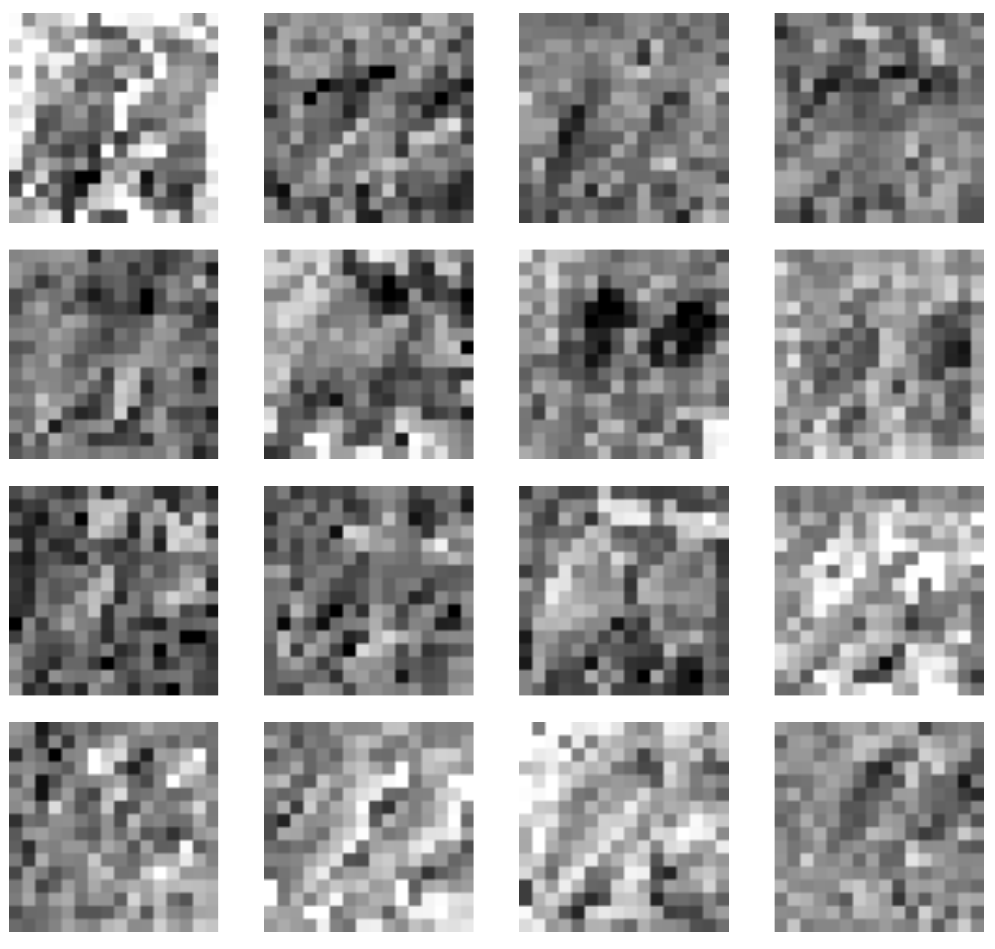
\includegraphics[width=5cm]{Figures/original.png}
    \caption{Visualization of DINOv2 Features.}
    \label{fig:dinov2features}
\end{figure}

\paragraph{Ablation on BeiT-2's Feature Representation}
BeiT-2's intermediary representation consists of four feature maps from attention blocks 3,5,7, and 11. These four feature maps are input to BeiT-2's semantic segmentation head and upon inspection, it is clear that feature maps from blocks 3 and 5 contain considerably less semantic features than in blocks 7 and 11 (see Figure \ref{fig:beit-features}). With this observation, we considered using just feature \#7 or just feature \#11, but found that these two settings were not as effective as applying an element-wise add across all feature maps as shown in Table \ref{tab:beit-feature-representations}.

\begin{table}[]
    \centering
    \begin{tabular}{c|c c}
    BeiT-2 Feature Representation & mIOU & BPP\\
    \hline
       standard (using features 3,5,7,11)  &  52.95 & 384\\
        only feature map from block \# 7 & 48.49 & 96 \\
        only feature map from block \# 11 & 54.01 & 96\\
        element-wise add all features & \textbf{54.74} & 96\\
    \end{tabular}
    \caption{BeiT-2 Feature Representations. The standard BeiT-2 feature representation consists of four feature maps from attention blocks 3,5,7, and 11. We consider what happens if we only use one feature map, or add all feature maps together.}
    \label{tab:beit-feature-representations}
\end{table}

% \textbf{Next Steps}
% From our BeiT classification experiments, we are successful at generating high compression ratios of $> 100:1$ using FSQ and standard integer quantization. In our next phase of this project, we will address the harder problem of compression for semantic segmentation.

% Additionally, handling variable-size images \& audio remains a key challenge in machine-oriented compression systems. For example, most image compression techniques automatically resize images to 224x244, which purposefully removes information prior to compression. Our results for feature compression indicate a promising path forward: by maintaining two representations (one fixed in size and another variable) which are jointly compressed, we can maintain good reconstruction quality and near-lossless performance on downstream tasks.

\section{Conclusion}
We present an analysis of existing full-input image compression pipelines and quantitatively compare conventional lossy compression with state-of-the-art neural compression for a variety of machine perception tasks. Additionally, we show promising model-splitting compression results for both BeiT-2 and DINOv2 features, achieving a 588X compression ratio for BeiT-2 image classification with 1.2\% accuracy degradation and a 3X compression ratio for semantic segmentation with only a 1.24 point mIOU degradation. Using DINOv2, we achieve higher compression rates than JPEG at typical quality settings, while significantly simplifying its deployment. Overall, we advocate for feature compression over raw image compression since operation on the original signal increases the performance ceiling, while the model-splitting approach accelerates aspects of both training and inference.

\section{Individual Member Contribution}
Dan Jacobellis completed all the experiments related to full-input compression and DINOv2 experiments while Natalia Frumkin completed all experiments for BeiT-2. We had regular discussions regarding our results and worked together on the reports and video.


{\small
\bibliographystyle{ieee_fullname}
\bibliography{egbib}
}

\end{document}
